\documentclass[12pt,letterpaper]{article}

\usepackage[margin=1in]{geometry}
\usepackage{fontspec}
\setmainfont{Times New Roman}
\usepackage{setspace}
\usepackage{graphicx}
\usepackage{booktabs}
\usepackage{array}
\usepackage{float}
\usepackage{caption}
\usepackage{fancyhdr}
\usepackage{ragged2e}
\usepackage{indentfirst}
\usepackage{hyperref}

\graphicspath{{../outputs/}{../outputs/resnet18_robust/}}
\hypersetup{colorlinks=false,pdfborder={0 0 0}}

\pagestyle{fancy}
\fancyhf{}
\fancyhead[C]{INDENG 1/242B Final Project Report}
\fancyfoot[C]{Robust Traffic Sign Recognition Under Visual Corruptions}
\renewcommand{\headrulewidth}{0pt}
\renewcommand{\footrulewidth}{0pt}

\captionsetup{
  font={small},
  labelfont=normalfont,
  textfont=normalfont,
  justification=centering,
  labelsep=period
}

\setlength{\parindent}{0.5in}
\setlength{\parskip}{0pt}
\setlength{\emergencystretch}{3em}
\RaggedRight
\sloppy
\doublespacing

\title{\vspace{-0.35in}\textbf{\fontsize{16}{20}\selectfont Robust Traffic Sign Recognition Under Visual Corruptions}}
\author{}
\date{}

\begin{document}
\maketitle
\vspace{-0.45in}

Course: INDENG 1/242B Final Project

Team: [Insert names]

Interactive demo: \url{https://huggingface.co/spaces/Theo9598/gtsrb-reliability-workbench}

GitHub appendix: \url{https://github.com/Theo9598/gtsrb-reliability/blob/master/APPENDIX.md}

Presentation recording: [Insert recording link before Gradescope submission]

\section*{Abstract}
We study traffic sign recognition as a 43-class image classification task using the German Traffic Sign Recognition Benchmark (GTSRB). To match the course emphasis on building a model, we train our own convolutional neural network from scratch and compare it against two stronger training conditions: the same CNN with RandAugment and MixUp, and an ImageNet-pretrained ResNet18 with RandAugment and MixUp. The custom CNN reaches 58.99\% clean test accuracy, the custom CNN with robust training reaches 54.43\%, and the final ResNet18 reaches 98.76\% accuracy and 98.33\% macro F1. This result shows that advanced augmentation is not automatically beneficial for a small from-scratch model, but is highly effective when paired with a higher-capacity pretrained backbone. We also run a CNN ablation study: removing BatchNorm drops clean test accuracy to 19.21\%, and removing Dropout drops it to 39.05\%, showing why these course concepts matter. Because traffic sign recognition is safety-relevant, we evaluate visual corruptions, apply temperature scaling to reduce expected calibration error from 6.36\% to 3.04\%, and deploy a Streamlit demo with upload, corruption, top-5 prediction, and Grad-CAM features.

\section{Motivation and Learning Problem}
Traffic sign recognition is a core perception task for driver-assistance and autonomous vehicle research. A useful classifier should perform well not only on clean benchmark images, but also under realistic image degradation caused by motion, compression, lighting, camera quality, or weather. A wrong prediction on a stop sign, no-entry sign, or speed-limit sign could be dangerous if a downstream system over-trusts the classifier.

We formulate the task as supervised multiclass classification. Each input $X_i$ is a cropped RGB traffic sign image, and each label $Y_i$ is one of 43 GTSRB classes. The model $f_\theta(X_i)$ outputs 43 logits, which are converted to class probabilities using softmax. The prediction is the class with maximum probability. We train using multiclass cross-entropy with regularization:
\[
\min_\theta \frac{1}{N}\sum_i L(f_\theta(X_i),Y_i)+R(\theta),
\]
where $R(\theta)$ includes weight decay, data augmentation, MixUp, and validation-based checkpoint selection.

\section{Data}
We use the Hugging Face GTSRB dataset \texttt{tanganke/gtsrb}, with 26,640 training images and 12,630 official test images over 43 classes. All model comparisons use the same data protocol: the original training split is divided once into a 22,644-image training subset and a 3,996-image validation subset using a stratified split with seed 242 and validation fraction 0.15. The official 12,630-image clean test split is never used for training or validation checkpoint selection; it is used only for final evaluation. Images are resized to 96 by 96 pixels and normalized using ImageNet mean and standard deviation to match the pretrained ResNet18 backbone.

The dataset contains cropped signs, so this project studies classification rather than object detection in full road scenes. To measure reliability, we evaluate on both locally generated corruptions and the dataset's corrupted splits. Local corruptions include Gaussian noise, blur, JPEG compression, pixelation, and low contrast. The provided corrupted splits include contrast, Gaussian noise, impulse noise, JPEG compression, motion blur, pixelate, and spatter. This lets us compare clean benchmark performance to performance under degraded visual conditions.

\section{Methodology}
The project uses three model conditions so that the report includes a course-aligned model, a training-method comparison, and an advanced transfer-learning model. The course-aligned model is a custom CNN trained from scratch, meaning all convolutional, BatchNorm, and classifier weights are randomly initialized and learned only from the GTSRB training set. We then train the same CNN with RandAugment and MixUp to test whether the robust training method helps the self-built model. Finally, we train an ImageNet-pretrained ResNet18 with the same robust training strategy to test how much transfer learning and model capacity improve performance.

\subsection*{Custom CNN architecture.}
The custom CNN follows the standard lecture pipeline for image classification: convolutional filters produce feature maps, ReLU adds nonlinearity, pooling reduces spatial resolution, BatchNorm stabilizes intermediate activations, Dropout regularizes the classifier, and a final linear layer outputs 43 logits. The logits are trained with multiclass cross-entropy, which combines the softmax probability model with the negative log-likelihood of the true traffic sign class.

\begin{table}[H]
\centering
\caption{Custom CNN architecture implemented from scratch.}
\footnotesize
\begin{tabular}{p{0.75in}p{2.45in}p{0.95in}p{1.55in}}
\toprule
Stage & Layer(s) & Output & Course Concept \\
\midrule
Input & RGB image resized to $96 \times 96$ & 3 channels & Image tensor \\
Block 1 & Conv2d 3$\rightarrow$32, BatchNorm, ReLU, MaxPool & 32 maps & Filters, activation, pooling \\
Block 2 & Conv2d 32$\rightarrow$64, BatchNorm, ReLU, MaxPool & 64 maps & Hierarchical features \\
Block 3 & Conv2d 64$\rightarrow$128, BatchNorm, ReLU, MaxPool & 128 maps & Deeper visual patterns \\
Block 4 & Conv2d 128$\rightarrow$256, BatchNorm, ReLU, AdaptiveAvgPool & 256 pooled features & Global aggregation \\
Classifier & Flatten, Dropout 0.35, Linear 256$\rightarrow$43 & 43 logits & Regularization and classification \\
\bottomrule
\end{tabular}
\end{table}

Both models are trained with minibatches and multiclass cross-entropy. For the custom CNN, the goal is to demonstrate the mechanisms learned in class: convolutional filters learn local visual patterns, pooling reduces spatial size, ReLU introduces nonlinearity, BatchNorm stabilizes activation distributions, Dropout regularizes the classifier, and softmax converts logits into class probabilities. For the ResNet18 model, we use AdamW, weight decay, a cosine learning-rate schedule, an initially frozen backbone, and later end-to-end fine-tuning.

Our advanced methodology beyond the standard CNN pipeline is robust training with RandAugment and MixUp. RandAugment randomly applies image transformations so the model learns useful invariances. MixUp forms convex combinations of images and labels, encouraging smoother decision boundaries and reducing overconfident memorization. We also add two deployment-aware components: temperature scaling calibrates confidence by rescaling logits before softmax, and Grad-CAM visualizes which image regions influence the prediction.

\section{Results}
The custom CNN was trained for 12 epochs from scratch. It reached 78.03\% validation accuracy and 58.99\% clean test accuracy. The same CNN trained with RandAugment and MixUp reached 66.09\% validation accuracy and 54.43\% clean test accuracy. This lower result is useful experimentally: strong augmentation and MixUp regularize the model, but the small CNN does not have enough capacity or training time to benefit from them under the current setting. The final ResNet18 model trained for 25 epochs on an NVIDIA GeForce RTX 2080 Ti and reached 99.97\% validation accuracy, 98.76\% clean test accuracy, and 98.33\% macro F1. These results are comparable because every row uses the same stratified training/validation split and the same official clean test set; only the model and training method change.

\begin{table}[H]
\centering
\caption{Main model and robust-training comparison.}
\scriptsize
\setlength{\tabcolsep}{3pt}
\begin{tabular}{p{1.35in}p{0.52in}p{0.62in}p{1.58in}p{1.05in}}
\toprule
Model & Pretrained? & Robust training? & Metrics (\%) & Interpretation \\
\midrule
Custom CNN & No & No & Val 78.03; Test 58.99; F1 39.26 & Course baseline \\
Custom CNN + RandAugment/MixUp & No & Yes & Val 66.09; Test 54.43; F1 34.25 & Strong regularization hurt this small model \\
ResNet18 + RandAugment/MixUp & Yes & Yes & Val 99.97; Test 98.76; F1 98.33 & Final high-performing model \\
\bottomrule
\end{tabular}
\end{table}

\begin{figure}[H]
\centering
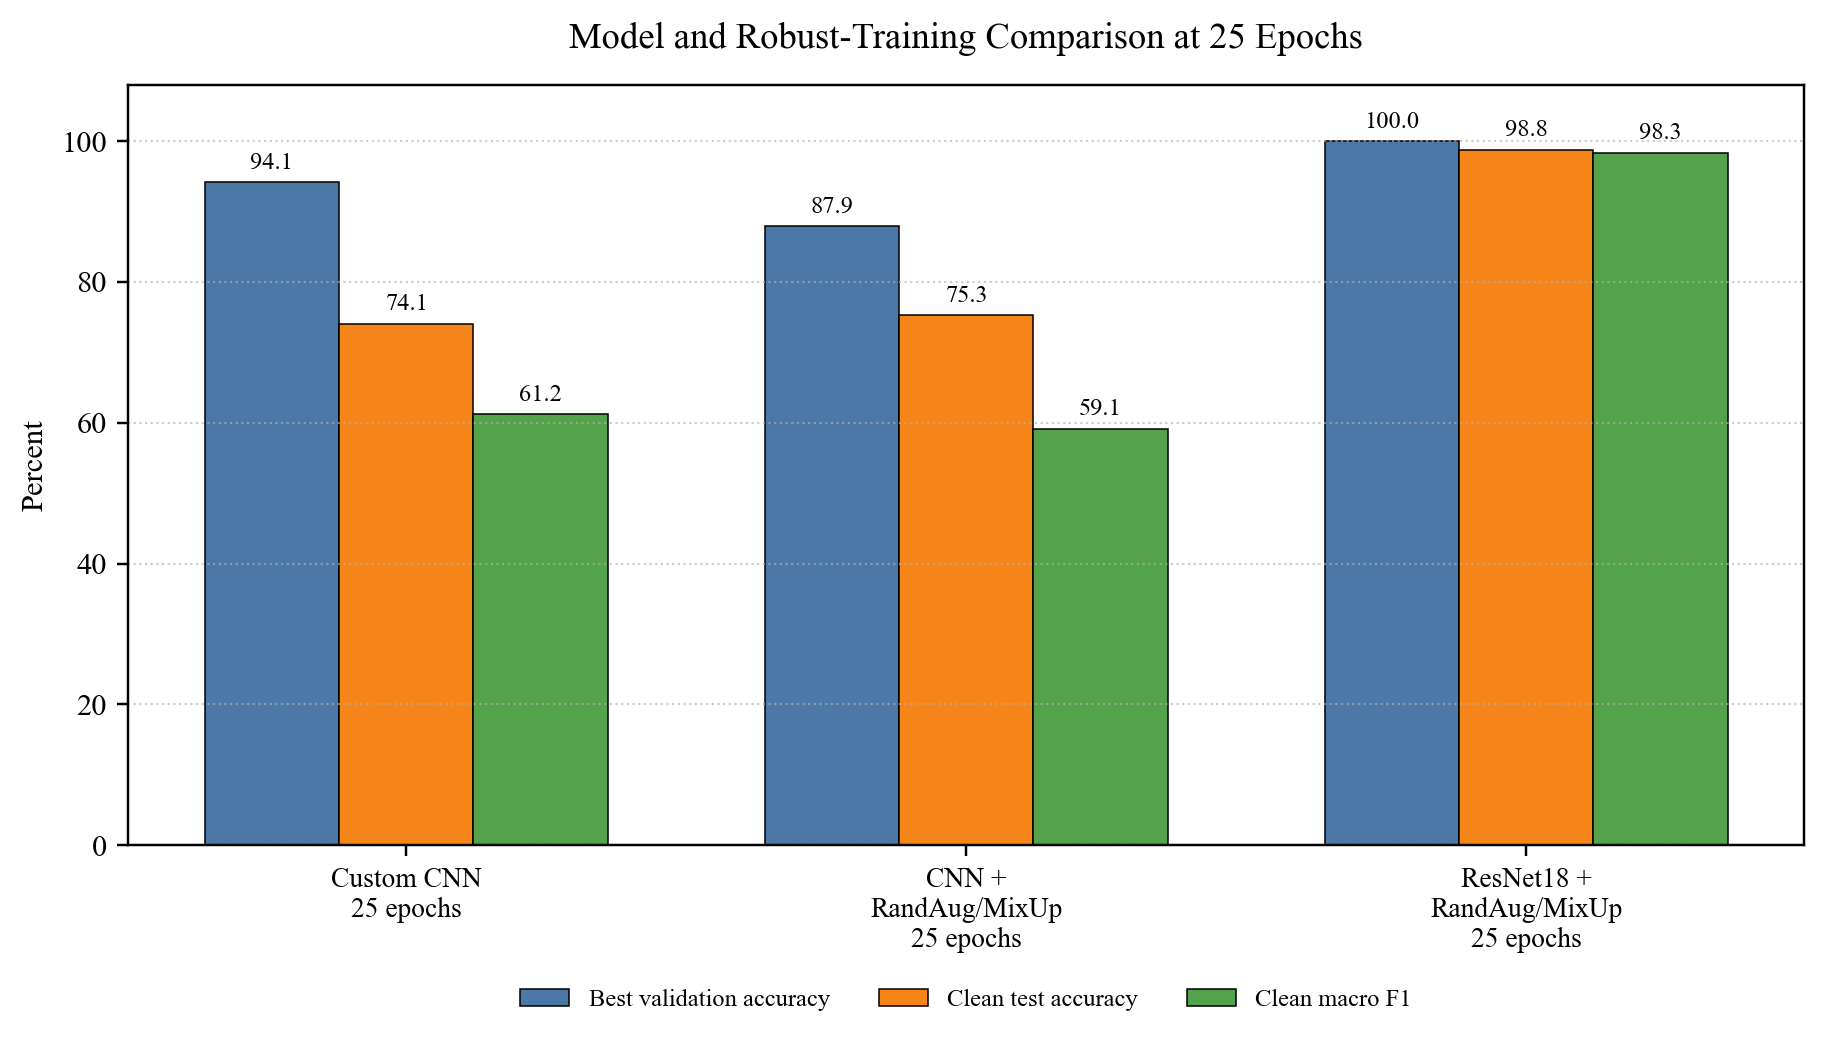
\includegraphics[width=5.7in]{cnn_augmix_resnet_comparison.png}
\caption{Custom CNN, robustly trained CNN, and robustly trained ResNet18 comparison.}
\end{figure}

Table 2 reports the main comparison directly. The first row is the self-built course model. The second row isolates the effect of adding RandAugment and MixUp to the same CNN architecture. In this run, robust training reduces clean-test accuracy by 4.56 percentage points, which suggests that the small from-scratch CNN is under-capacity or under-trained for this stronger regularization. The third row shows that the same robust training idea is much more effective when paired with a pretrained ResNet18 backbone, improving clean-test accuracy by 39.77 percentage points over the plain custom CNN.

\begin{table}[H]
\centering
\caption{Custom CNN ablation results.}
\footnotesize
\begin{tabular}{p{1.45in}p{0.75in}p{2.45in}p{1.15in}}
\toprule
Model & Pretrained? & Metrics (\%) & Delta vs Full CNN \\
\midrule
Full custom CNN & No & Val 78.03; Test 58.99; F1 39.26 & Baseline \\
No BatchNorm & No & Val 20.85; Test 19.21; F1 6.02 & -39.78 pp \\
No Dropout & No & Val 50.03; Test 39.05; F1 21.06 & -19.94 pp \\
\bottomrule
\end{tabular}
\end{table}

The ablation in Table 3 supports the course concepts inside the custom CNN. Removing BatchNorm causes the largest drop, which means normalization is important for stable training in this architecture. Removing Dropout also hurts performance, showing that regularization helps the classifier generalize beyond the training split.

\begin{figure}[H]
\centering

\includegraphics[width=5.7in]{training_curves.png}
\caption{Training and validation loss/accuracy curves.}
\end{figure}

On the clean official GTSRB test set, the model performs strongly:

\begin{table}[H]
\centering
\footnotesize
\begin{tabular}{p{2.7in}p{2.3in}}
\toprule
Metric & Value \\
\midrule
Accuracy & 98.76\% \\
95\% bootstrap CI for accuracy & 98.56\%--98.95\% \\
Macro F1 & 98.33\% \\
ECE before calibration & 6.36\% \\
ECE after temperature scaling & 3.04\% \\
Learned temperature & 0.8592 \\
\bottomrule
\end{tabular}
\end{table}

Robustness testing gives a more complete picture:

\begin{table}[H]
\centering
\scriptsize
\begin{tabular}{p{1.35in}p{1.35in}p{0.9in}p{0.9in}}
\toprule
Evaluation split & Source & Accuracy & Macro F1 \\
\midrule
Clean test & Clean & 98.76\% & 98.33\% \\
Gaussian noise & Local corruption & 84.57\% & 84.44\% \\
Blur & Local corruption & 62.61\% & 62.21\% \\
JPEG compression & Local corruption & 85.91\% & 84.99\% \\
Pixelate & Local corruption & 36.30\% & 32.89\% \\
Low contrast & Local corruption & 99.42\% & 98.00\% \\
Contrast & HF corrupted split & 98.42\% & 97.86\% \\
Gaussian noise & HF corrupted split & 88.25\% & 87.53\% \\
Impulse noise & HF corrupted split & 84.24\% & 83.44\% \\
JPEG compression & HF corrupted split & 96.05\% & 95.14\% \\
Motion blur & HF corrupted split & 97.93\% & 97.14\% \\
Pixelate & HF corrupted split & 96.79\% & 95.83\% \\
Spatter & HF corrupted split & 91.91\% & 90.20\% \\
\bottomrule
\end{tabular}
\end{table}

The model is robust to several benchmark corruptions, especially contrast, motion blur, JPEG compression, and low contrast. However, severe local pixelation is a major weakness: accuracy drops to 36.30\%. This likely removes fine details such as digits, arrows, and sign boundaries that distinguish similar classes. Thus, the project produces a scientifically useful result: the model is strong on clean and many corrupted images, but not reliable under every degradation.

\begin{figure}[H]
\centering

\includegraphics[width=5.8in]{robustness_by_corruption.png}
\caption{Accuracy under clean and corrupted evaluation splits.}
\end{figure}

Calibration also improves meaningfully. Expected calibration error decreases from 6.36\% to 3.04\% after temperature scaling, which makes predicted confidence more aligned with empirical correctness. This matters because high confidence should not be interpreted as a guarantee of safety.

\begin{figure}[H]
\centering

\includegraphics[width=4.7in]{reliability_diagram.png}
\caption{Reliability diagram after temperature scaling.}
\end{figure}

\section{Interactive Tool and Bonus Component}
We deploy a Streamlit workbench on Hugging Face Spaces: \url{https://huggingface.co/spaces/Theo9598/gtsrb-reliability-workbench}. The tool lets users upload a traffic sign image, view top-5 predictions, apply realistic corruptions, adjust calibration temperature, and inspect Grad-CAM heatmaps. This interaction directly supports the project thesis: users can test whether a prediction remains stable when the image is degraded, rather than only seeing one clean-image classification result. The complete appendix, commands, source-code map, and additional diagnostic figures are maintained in the GitHub repository appendix: \url{https://github.com/Theo9598/gtsrb-reliability/blob/master/APPENDIX.md}.

\section{Safety, Security, and Ethics}
This project should be treated as an educational prototype, not a deployable autonomous driving component. It classifies cropped signs but does not detect signs in full road scenes. It also does not handle occlusion, night driving, unusual weather, camera motion, vandalized signs, adversarial stickers, or map context.

False predictions can be safety-critical. Misclassifying a stop sign, no-entry sign, or speed limit could cause unsafe downstream behavior if used without safeguards. Domain shift is also important because GTSRB uses German signs; results may not transfer to other countries or rare sign variants. The corruption experiments show that high clean accuracy does not guarantee robustness, especially under severe resolution loss.

A real deployment would require uncertainty thresholds, out-of-distribution detection, redundant sensors, human oversight, extensive field testing, and regulatory review. For this reason, the demo includes an educational-use disclaimer.

\section{Conclusion}
This project applies deep learning methodology to a real image classification problem and extends it with robustness, calibration, interpretability, and deployment analysis. The custom CNN architecture demonstrates course concepts directly: convolution, ReLU, pooling, BatchNorm, Dropout, softmax-style multiclass classification, and cross-entropy training. The comparison between plain CNN, CNN with RandAugment/MixUp, and ResNet18 with RandAugment/MixUp shows that robust training is not a magic switch; it works best when the model has enough representational capacity and useful pretrained features. The ablation study shows that BatchNorm and Dropout materially affect the self-built CNN. The fine-tuned ResNet18 trained with RandAugment and MixUp achieves 98.76\% clean test accuracy and 98.33\% macro F1 on GTSRB. Calibration reduces ECE from 6.36\% to 3.04\%, and corruption testing reveals the model's strengths and limitations. The main conclusion is that strong clean performance is achievable, but reliability requires explicit model comparison, ablation, robustness testing, and safety analysis.

\end{document}
